\documentclass{article}
\usepackage[margin=0.5in]{geometry}
\usepackage{graphicx}
\usepackage[font={small,it}]{caption}
\usepackage{wrapfig}
\usepackage{Sweave}
\begin{document}
\Sconcordance{concordance:latexStatisticsCoursework.tex:latexStatisticsCoursework.Rnw:%
1 7 1 50 0 1 15 6 1 1 4 1 1 1 74 19 1 1 7 9 1 1 19 20 1 5 0 2 1 1 5 1 1 1 6 1 1 %
1 17 15 1}



\title{Statistics Coursework}
\author{Alun Meredith}
\maketitle
\section{Reading data}
Downloaded fish.txt, data about the catch of a hypothetical fishing fleet from:\\"http://www.edshare.soton.ac.uk/view/courses/COMP6235/2015.html" on Sun Oct 25 20:20:01 2015. 
\begin{Schunk}
\begin{Sinput}
> readLines("fish.txt", 5)
\end{Sinput}
\begin{Soutput}
[1] "15.25 2.79 " "13.45 2.69 " "5.58 2.20 "  "7.17 3.21 "  "13.81 2.12 "
\end{Soutput}
\end{Schunk}
From reading the first 5 lines of the file we can see that the data is 2 numeric columns. Each variable is seperated by a single whitespace, there is no header and no apparent NA characters or comment/escape characters. As such we can use the default values of read.table, including the col.names argument to name the variables.
\section{Visualising Data}
\begin{figure}[h]
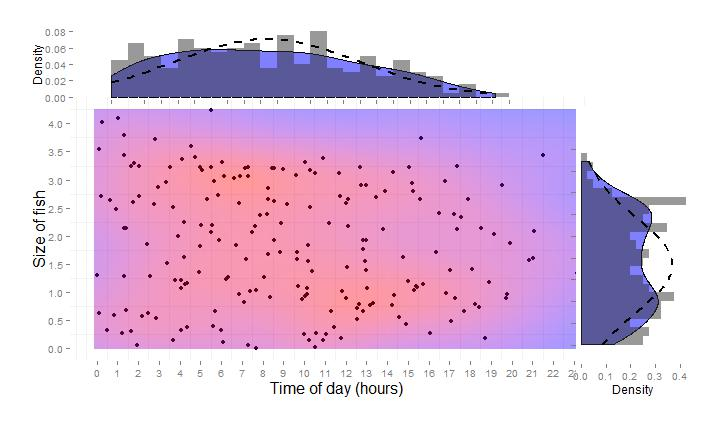
\includegraphics[width=\linewidth]{figure1.jpg}
\caption{\textbf{Bottom Left}: Scatter graph of size of fish caught vs time of day (hours), coloured background demonstrating gaussian kernel 2d density \textbf{Right}: Histogram showing distribution of size of fish caught with gaussian kernel density plot overlayed \textbf{Top}: Histogram showing time of day fish caught overlayed by density plot, dashed line shows normal distributions for equal mean and standard deviation}
\label{fig:1}
\end{figure}
% latex table generated in R 3.2.1 by xtable 1.7-4 package
% Sun Oct 25 20:20:02 2015
\begin{table}[ht]
\centering
\begin{tabular}{rrrrrrrrrrr}
  \hline
 & min & Q1 & median & Q3 & max & mean & s.dev & skewness & kurtosis & geometric mean \\ 
  \hline
sizeSummary & 0.01 & 0.94 & 1.83 & 2.74 & 4.23 & 1.84 & 1.08 & 0.09 & -1.17 & 1.37 \\ 
  timesSummary & 0.01 & 4.88 & 8.95 & 13.22 & 23.16 & 9.39 & 5.66 & 0.25 & -0.89 & 6.79 \\ 
   \hline
\end{tabular}
\caption{Numeric summary statistics for Time and Size Distributions} 
\end{table}
\section{Analysing Distributions}

By looking at the above summary statistics and the density distributions in figure \ref{fig:1}, we can see some interesting features of the distributions. The time fish were caught was very broard with high standard deviation. There is some skewness which can be seen clearly in the plot. This is fairly surprising as you would expect the density at 12:01 to be approximately equal to the density at 11:59 in a cyclical manor. This suggests that an effect such as the data being recorded on a Saturday where no fishing is done on a Sunday is occuring, but requires more domain knowledge to analyse fully.

The distribution of fish sizes (right hand density plot in figure \ref{fig:1}) shows a distribution which is visibly bimodal. The standard deviation covers 51.18\% of the data range, which is greater than the wide flat times data of 48.9, this is probably due to the bimodal distributions. Both the mean and median sits between the two peaks and there is negligible skewness because the peaks are approximately symmetric and equal in size. 

\subsection{Confidence Intervals}


\begin{wrapfigure}[11]{R}{6cm}
  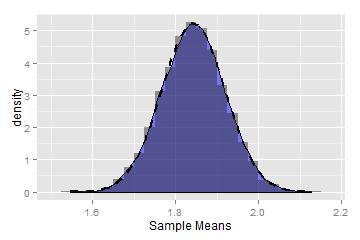
\includegraphics[width=0.9\linewidth]{figure3.jpg}
  \caption{10000 sample means taken from fish size data, blue region is density, dashed line shows normal distribution with equal mean and variance.}
  \label{fig:three}
\end{wrapfigure}

Both of the distributions are clearly not normally distributed as shown by the dashed normal distributions (with same mean/variance) shown in the figure. This introduces some complexity in producing confidence intervals. For the time caught confidence interval it is possible to closely approximate the normal distribution by transforming the data.

In order to evaluate a confidence interval from these non-standard distributions a method called bootstrapping is used. As shown in fig.\ref{fig:three} by resampling our data and plotting the means we get a distribution that closely approximates the normal distribution via the central limit theorem. The mean of a sample distribution approximates the mean of the population it was sampled from. By calculating a confidence interval for this mean we can estimate a 95\% confidence interval for the population of:

% latex table generated in R 3.2.1 by xtable 1.7-4 package
% Sun Oct 25 20:20:03 2015
\begin{table}[ht]
\centering
\begin{tabular}{rrr}
  \hline
  \hline
SizeConfidence & 1.69 & 1.99 \\ 
  TimeConfidence & 8.60 & 10.17 \\ 
   \hline
\end{tabular}
\caption{Bootstrapped 95 percent confidence intervals} 
\end{table}
\section{Codependency}

The central figure above shows a scatter of size of fish and time of day. It is hard to identify any dependencies in the data visually but it looks as though it may be slightly weakly correlated. After numerical analysis we can see a covariance of -0.78 and a Pearson product-moment correlation of -0.13.

The correlation is very weak but one explanation could be that you would expect the bigger fish to be easier to catch, therefore the population of bigger fish in the water shrinks over the course of the day. We would need more domain knowledge to conclude an effect like this. For instance if the fishing is taking place over a larger area (larger population of fish) then the fish caught early in the day will have quite a small effect on the ammount left at the end of the day. 

\section{Intervals}

Splitting the times into 24 intevals corresponding to each hour of the day we can show the interval of time with the highest rate of catch is 12:00 to  13:00. The interval with the largest average size of fish caught is 21:00 to 22:00. 

Although this period has the largest average size of fish caught, it is not what would be initially expected considering the negative correlation calcualted. If each interval is inspected individually, this is an outlier to the general trend in which that the first third of the day averages around 2 and the last half the day is almsot entirely below 2 (with 2 exceptions). 
\end{document}
